% -*- TeX:Rnw -*-
% ----------------------------------------------------------------
% .R Sweave file  ************************************************
% ----------------------------------------------------------------
%%
%\documentclass[a4paper,12pt,english]{article}
\documentclass[a4paper,12pt,slovene]{article}
\newcommand{\SVNRevision}{$Rev:   $}
\newcommand{\SVNDate}{$Date::            $}
\usepackage{babel}
\input{abpkg}
\input{abcmd}
\input{abpage}
\usepackage{pgf,pgfarrows,pgfnodes,pgfautomata,pgfheaps,pgfshade}
\usepackage{amsmath,amssymb}
\usepackage{colortbl}
\usepackage{Sweave}
\input{mysweave}


\setkeys{Gin}{width=0.7\textwidth}
\usepackage{lmodern}
\input{abfont}
%\SweaveOpts{keep.source=true}
%\setkeys{Gin}{width=0.8\textwidth} % set graphicx parameter
% ----------------------------------------------------------------
%\makeindex
\begin{document}
%% Sweave settings for includegraphics default plot size (Sweave default is 0.8)
%% notice this must be after begin{document}
%%% \setkeys{Gin}{width=0.9\textwidth}
% ----------------------------------------------------------------
\title{Verjetnostne porazdelitve}
\author{A. Blejec}
%\address{}%
%\email{}%
%
%\thanks{}%
%\subjclass{}%
%\keywords{}%

%\date{}%
%\dedicatory{}%
%\commby{}%
\maketitle
% ----------------------------------------------------------------
\begin{abstract}
Opisanih je nekaj diskrtenih in zveznih verjetnostnih porazdelitev:
Bernoullijeva, enakomerna diskretna, binomska, Poissonova, geometrijska (Pascalova), negativna binomska, Poissonova (za �as in prostor), eksponentna in gama.
\end{abstract}
% ----------------------------------------------------------------
\setlength{\parskip}{0pt}
%\begin{spacing}{0.5}
\tableofcontents
%\end{spacing}
\setlength{\parskip}{\baselineskip}
\pagestyle{plain}
% ----------------------------------------------------------------
\clearpage
\section{Bernoulli-jeva porazdelitev}
Diskretna porazdelitev, ki opisuje verjetnost Bernoullijevega poskusa, ki ima izida \emph{1} in \emph{0} z verjetnostma $p$ in $1-p$:

\begin{displaymath}
X\sim
\left( \begin{array}{cc}
            1 & 0 \\
            p & 1-p
\end{array} \right)
\end{displaymath}

Pogosto pi�emo $1-p=q$

$$E(X)=p$$
$$V(X)=p\cdot(1-p)=pq$$

\vspace{2cm}
Dve raz�iritvi:

\begin{itemize}
  \item raz�iritev na ve� mo�nih izidov $1, 2, 3, \ldots, m$
  \item poskus ve�krat ponovimo, tako dobimo zaporedje B. poskusov
\end{itemize}

\clearpage
\section{Diskretna enakomerna porazdelitev}

�e raz�irimo Bernoullijev poskus z dva na poskus z $m$ enakomo�nimi izidi
$1,2,3,...,m$, ki imajo vsi enako verjetnost $p=1/m$ dobimo diskretno enakomerno porazdelitev
$$
X\sim
\left( \begin{array}{ccccc}
         1 & 2 & 3 & \ldots& m \\
         p & p & p & \ldots & p
       \end{array}
\right)
$$

$$E(X)=(m+1)/2$$
$$V(X)=\frac{m^2-1}{12}$$




Za $m=6$ lahko vzamemo kot model igralno kocko:
$$E(X)=3.5$$
$$V(X)=2.917$$

\begin{Schunk}
\begin{Soutput}
  [1] 4 2 2 5 6 5 4 6 3 5 6 5 6 4 1 1 2 6 2 1 3 5 2 2 1 2 3 1 5 4 2 3
 [33] 2 6 4 1 2 4 2 2 4 3 5 4 2 3 5 4 2 1 5 6 3 1 1 2 3 5 1 1 1 5 6 6
 [65] 3 6 4 5 1 5 4 6 3 1 3 1 2 4 1 2 3 5 4 5 3 3 5 3 2 3 4 2 4 5 2 6
 [97] 4 2 6 5 6 2 2 2 1 1 3 5 4 3 3 4 5 3 6 4 3 2 6 6
\end{Soutput}
\begin{Soutput}
Povpre�je: 3.408333
\end{Soutput}
\begin{Soutput}
Varianca : 2.764636
\end{Soutput}
\end{Schunk}

\begin{center}
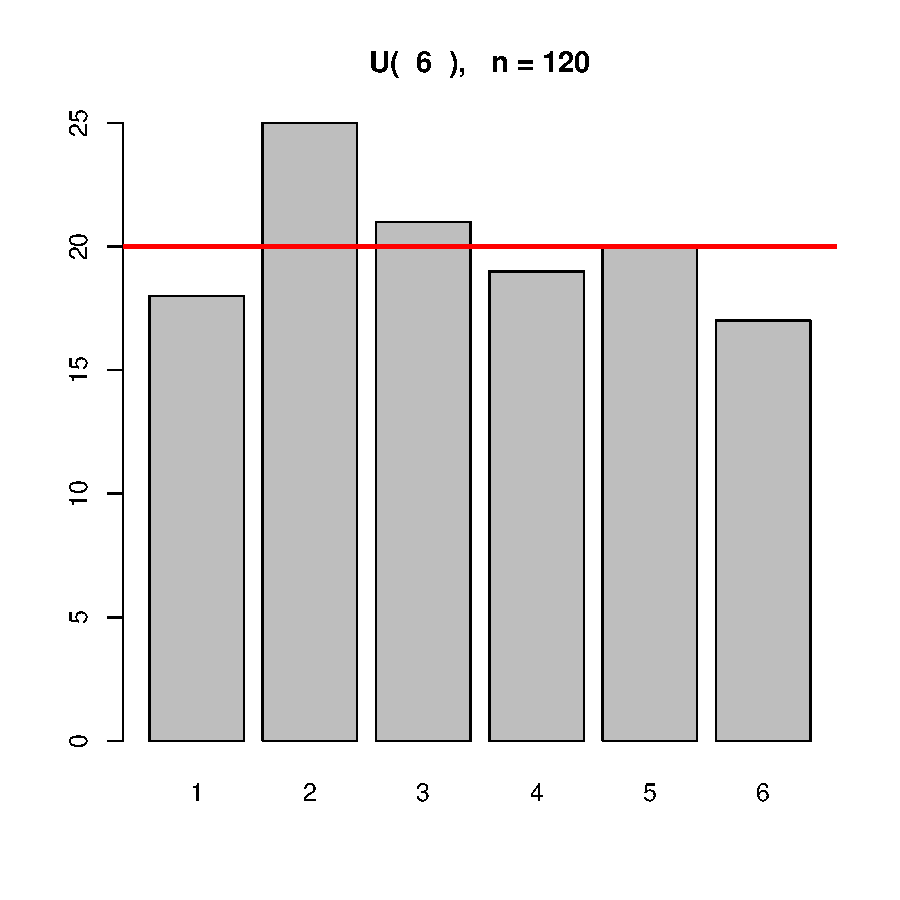
\includegraphics{./figs/porazdelitve-dunif}
\end{center}




\clearpage
\section{Eksponentna porazdelitev}
\emph{�akalni �as do prvega dogodka}, pri znanem povpre�nem pre�ivetvenem �asu $\beta=1/\lambda$ opisuje eksponentna porazdelitev ($\lambda$ je �tevilo dogodkov v enoti �asa, 'rate' ):

$$f(T)=\lambda e^{-\lambda T}=\frac{1}{\beta} e^{-\frac{T}{\beta}}$$

$$E(T)=\frac{1}{\lambda}=\beta$$
$$V(T)=\frac{1}{\lambda^2}=\beta ^2$$
Kumulativna porazdelitev (porazdelitvena funkcija)
$$F(t)=P(T\le t)= 1-e^{-\lambda t}$$
Krivulja pre�ivetja:
$$P(T>s+t|T>s)=P(T>t)=\overline{F}(t)=1-F(t)=e^{-\lambda t}$$

\begin{center}
\begin{Schunk}
\begin{Soutput}
Beta     : 0.2
 Lambda   : 5
 Povpre�je: 0.2037135
 Varianca : 0.03901648
\end{Soutput}
\end{Schunk}
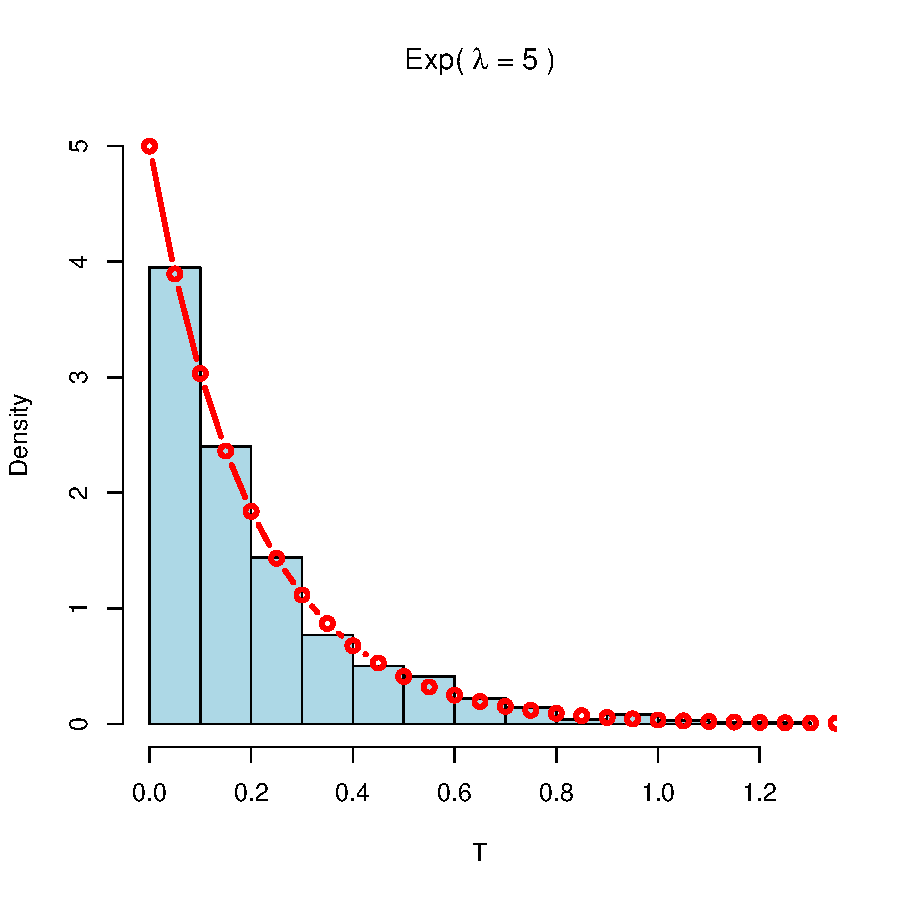
\includegraphics{./figs/porazdelitve-exp}
\end{center}

\clearpage
\section{Gama porazdelitev}

\emph{�akalni �as do r-tega dogodka}, pri znanem povpre�nem pre�ivetvenem
�asu $\beta$. Pre�ivetveni �as je v zvezi s �tevilom dogodkov v enoti �asa $\lambda$

$$f(T|r,\beta)=\frac{1}{\Gamma(r)\beta^r} T^{r-1} e^{-\frac{T}{\beta}}$$

$$E(T)=r \beta$$
$$V(T)=r \beta ^2$$

Pre�ivetveni �as $\beta$ je v zvezi s �tevilom dogodkov v enoti �asa $\lambda$:
$$\beta= 1 / \lambda.$$

Gostoto lahko zapi�emo tudi takole:

$$f(T|r,\lambda)=\frac{\lambda^r T^{r-1} e^{-T \lambda}}{\Gamma(r)} $$


\begin{center}
\begin{Schunk}
\begin{Soutput}
r        : 4
\end{Soutput}
\begin{Soutput}
lambda   : 5
\end{Soutput}
\begin{Soutput}
Povpre�je: 0.824374
\end{Soutput}
\begin{Soutput}
Varianca : 0.1656046
\end{Soutput}
\end{Schunk}
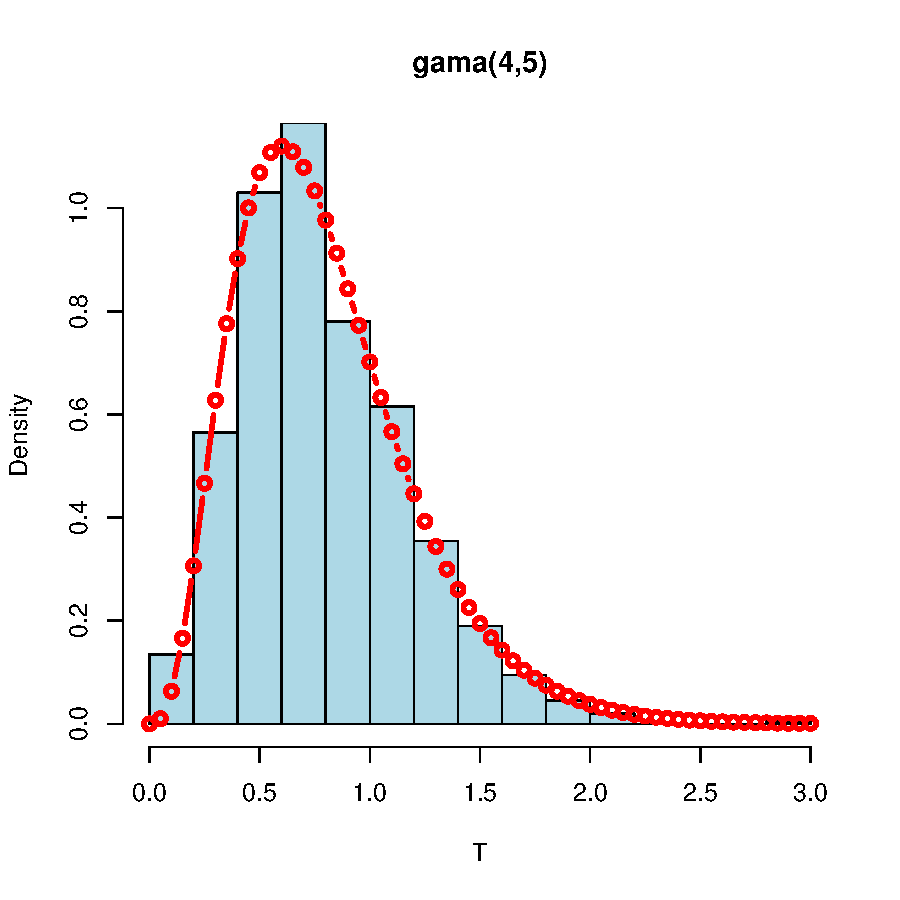
\includegraphics{./figs/porazdelitve-gama}
\end{center}

Opomba:\\
Eksponentna porazdelitev je Gama porazdelitev za $r=1$.
\clearpage
\section{Poissonova porazdelitev}

Poissonova porazdelitev opisuje porazdelitev �tevila dogodkov v �asu in prostoru, pri nekem
povpre�nem �tevilu dogodkov v enoti �asa ($\lambda$).

$$P [(N(t+ \tau) - N(t)) = k] = \frac{e^{-\lambda \tau} (\lambda
\tau)^k}{k!} \qquad k= 0,1,\ldots$$,
kjer $N(t + \tau) - N(t)$
predstavlja �tevilo dogodkov v intervalu $[t,t+\tau]$.






% ----------------------------------------------------------------
%\bibliographystyle{amsplain}
%\bibliography{}
\end{document}
% ----------------------------------------------------------------
